%%%%%%%%%%%%%%%%%%%%%%%%%%%%%%%%%%%%%%%%%
% Beamer Presentation
% LaTeX Template
% Version 1.0 (10/11/12)
%
% This template has been downloaded from:
% http://www.LaTeXTemplates.com
%
% License:
% CC BY-NC-SA 3.0 (http://creativecommons.org/licenses/by-nc-sa/3.0/)
%
%%%%%%%%%%%%%%%%%%%%%%%%%%%%%%%%%%%%%%%%%

%----------------------------------------------------------------------------------------
%	PACKAGES AND THEMES
%----------------------------------------------------------------------------------------

\documentclass{beamer}

\mode<presentation> {
	
	%\usetheme{default}
	%\usetheme{AnnArbor}
	%\usetheme{Antibes}
	%\usetheme{Bergen}
	%\usetheme{Berkeley}
	%\usetheme{Berlin}
	%\usetheme{Boadilla}
	%\usetheme{CambridgeUS}
	%\usetheme{Copenhagen}
	%\usetheme{Darmstadt}
	%\usetheme{Dresden}
	%\usetheme{Frankfurt}
	%\usetheme{Goettingen}
	%\usetheme{Hannover}
	%\usetheme{Ilmenau}
	%\usetheme{JuanLesPins}
	%\usetheme{Luebeck}
	\usetheme{Madrid}
	%\usetheme{Malmoe}
	%\usetheme{Marburg}
	%\usetheme{Montpellier}
	%\usetheme{PaloAlto}
	%\usetheme{Pittsburgh}
	%\usetheme{Rochester}
	%\usetheme{Singapore}
	%\usetheme{Szeged}
	%\usetheme{Warsaw}
	
	% As well as themes, the Beamer class has a number of color themes
	% for any slide theme. Uncomment each of these in turn to see how it
	% changes the colors of your current slide theme.
	
	%\usecolortheme{albatross}
	%\usecolortheme{beaver}
	%\usecolortheme{beetle}
	%\usecolortheme{crane}
	%\usecolortheme{dolphin}
	%\usecolortheme{dove}
	%\usecolortheme{fly}
	%\usecolortheme{lily}
	%\usecolortheme{orchid}
	%\usecolortheme{rose}
	%\usecolortheme{seagull}
	%\usecolortheme{seahorse}
	%\usecolortheme{whale}
	%\usecolortheme{wolverine}
	
	%\setbeamertemplate{footline} % To remove the footer line in all slides uncomment this line
	%\setbeamertemplate{footline}[page number] % To replace the footer line in all slides with a simple slide count uncomment this line
	
	%\setbeamertemplate{navigation symbols}{} % To remove the navigation symbols from the bottom of all slides uncomment this line
}


\makeatletter
\def\pdftex@driver{pdftex.def}
\ifx\Gin@driver\pdftex@driver
\def\pgfsys@color@unstacked#1{%
	\pdfliteral{\csname\string\color@#1\endcsname}%
}
\fi
\makeatother


\usepackage{graphicx} % Allows including images
\usepackage{booktabs} % Allows the use of \toprule, \midrule and \bottomrule in tables
\usepackage{xcolor}
\usepackage{listings}
\usepackage{fancybox}
\usepackage{mathtools}
\usepackage{multirow}
\usepackage{graphicx}
\usepackage{amssymb}
\usepackage[many]{tcolorbox}
\usepackage{amsmath}
%define a new block
\newenvironment<>{varblock}[2][\textwidth]{%
	\setlength{\textwidth}{#1}
	\begin{actionenv}#3%
		\def\insertblocktitle{#2}%
		\par%
		\usebeamertemplate{block begin}}
	{\par%
		\usebeamertemplate{block end}%
\end{actionenv}}

\setbeamertemplate{navigation symbols}{}

\newcommand{\g}{{\rm g}}
\newcommand{\bfr}{\mathbf{r}}
\newcommand{\I}{\mathrm{I}}
\newcommand{\R}{{\mathrm R}}
\newcommand{\hatf}{{\hat{f\,}\!}}
\newcommand{\hf}{\frac 12}
\newcommand{\ts}{\hspace{.06em}}
\newcommand{\tB}{{\tilde B}}
\newcommand{\tW}{{\tilde W}}
\newcommand{\tE}{{\tilde E}}
\newcommand{\tpsi}{{\tilde\psi}}


\DeclareMathOperator*{\argmax}{arg\,max}
\DeclareMathOperator*{\argmin}{arg\,min}
%----------------------------------------------------------------------------------------
%	TITLE PAGE
%----------------------------------------------------------------------------------------

\title[Bidding Algorithm Overview]{Bidding Algorithm Primer}
\author{Yuanlong Chen} 
\institute[Brand Auction] {
Brand Auction\\ % Your institution for the title page
	\medskip
}
\date{July 08, 2024} % Date, can be changed to a custom date

\begin{document}
	
	\newcommand{\SubItem}[1]{
		{\setlength\itemindent{15pt} \item[-] #1}
	}
	
	
	\begin{frame}
		\titlepage % Print the title page as the first slide
	\end{frame}
	
	%----------------------------------------------------------------------------------------
	
	\begin{frame}
		\frametitle{Agenda}
		

				\pause
			\begin{enumerate}	
				\item  \textbf{Bidding Products} \pause \\ 
				\item  \textbf{Auto-Bidding Algorithm} \pause \\
				\item  \textbf{Cost Cap Bidding Algorithm}
			\end{enumerate}

		
		
	\end{frame}


\begin{frame}
	\frametitle{Bidding Products}
	
	
\begin{block}{Three Major Bidding Products} 
	\pause
	\begin{enumerate}
		\item \textbf{Max Delivery (a.k.a no bid, lowest cost)}
		
		\textit{Advertiser's input}: budget, no ROI requirements
		
		\pause 
		\item \textbf{Cost Cap}
		
		\textit{Advertiser's input}: budget + cost cap (max CPX)
		
		\pause
		
		\item \textbf{Manual bidding(other companies) }
		
		\textit{Advertiser's input}: budget + fixed bid price
	\end{enumerate}
\end{block} \pause


\end{frame}
	
	
	%----------------------------------------------------------------------------------------
	
	\begin{frame}
		\frametitle{Auto Bidding Algorithm}
		\begin{block}{Formulation(use CPC ads as example)}
		\begin{displaymath}
			\begin{aligned}
				&\max_{x_t} \sum_{t=1}^{T} x_t \cdot r_t \quad \text{s.t.} \quad  \sum_{t=1}^{T} x_t \cdot c_t \leq B \\
				\text{where} \quad & \\
				& t  - \text{t-th auction opportunity} \\
				& T - \text{total auction opportunity} \\
				& r_t - \text{pctr at } t \\
				& c_t - \text{cost at } t \\
				& B - \text{total budget} \\
				& x_t - \text{indicator whether t-th auction win or lose, } x_t \in \{0, 1\}
			\end{aligned}
		\end{displaymath}
	\end{block}
	\end{frame}
	
	
	
		%----------------------------------------------------------------------------------------
	
	\begin{frame}
		\frametitle{Auto Bidding Algorithm}
		\pause 
		\begin{block}{Optimal Bidding Formula} 
			\pause
			Auction Mechanism: assume we use second price auction, then
			\[ 	x_t = \mathbf{1}_{\left\{ \text{ecpm}_t > c_t \right\}} \quad \text{where} \quad \text{ecpm}_t = b_t * r_t\] \pause
	
	\textbf{Idea}:  use primal-dual + online gradient descent to derive an optimal bidding formula for auto-bidding campaigns 
		\end{block}
		
	\end{frame}
	
	%----------------------------------------------------------------------------------------
	
		\begin{frame}
		\frametitle{Auto Bidding Algorithm}

		\begin{block}{Optimal Bidding Formula(cont'd)} 
			\pause
			
			\textbf{STEP 1: Write Lagrangian}
			
			\[
			\mathcal{L}(x_t, \lambda) = \sum_{t=1}^{T} x_t r_t + \lambda \left( B - \sum_{t=1}^{T} x_t c_t \right)
			\]
			\[
			= \sum_{t=1}^{T} x_t (r_t - \lambda c_t) + \lambda B
			\]
		
		\end{block}
		
	\end{frame}
	
	%----------------------------------------------------------------------------------------
	
	\begin{frame}
		\frametitle{Auto Bidding Algorithm}
		
		\begin{block}{Optimal Bidding Formula(cont'd)} 
			
			\textbf{STEP 2: Derive dual problem}
			
			\[
			\mathcal{L}^*(\lambda) = \max_{x_t} \mathcal{L}(x_t, \lambda)
			\]
			\[
			= \sum_{t=1}^{T} (r_t - \lambda c_t)_+ + \lambda B
			\]
			
			where \((z)_+ = \max(0, z)\) (a.k.a ReLU)

		\end{block}
		
	\end{frame}
	
	%----------------------------------------------------------------------------------------
	
\begin{frame}
	\frametitle{Auto Bidding Algorithm}
	
	\begin{block}{Optimal Bidding Formula(cont'd)} 
		
	\textbf{STEP 3: Solve dual problem}
	
	\[
	\lambda^* = \min_{\lambda \geq 0} \mathcal{L}^*(\lambda)
	\]
	
	\[
	\Rightarrow \text{ecpm}_t^* = \frac{r_t}{\lambda^*}
	\]
	i.e.
	\[
	b_t^* \cdot r_t = \frac{r_t}{\lambda^*} \Rightarrow b_t^* = \frac{1}{\lambda^*}
	\]
	
	
	\textit{Note: this is true for all incentive compatible auctions}

		
	\end{block}

	\pause

	\begin{tcolorbox}[colframe=blue,colback=blue!5!white]
		\begin{center}
				\textbf{Conclusion:} optimal bid is constant bid
		\end{center}
	\end{tcolorbox}
	
\end{frame}

%----------------------------------------------------------------------------------------
	
	


\begin{frame}
	\frametitle{Auto Bidding Algorithm}
	
	\begin{block}{How To Find Optimal Bid $b^*$} 
		
		(From KKT condition) $b^*$ is the bid level that exactly depletes the budget, i.e.,
		\[
		\sum_{t=1}^{T} x_t c_t \leq B \implies \sum_{t=1}^{T} x_t c_t = B
		\] \pause
		
		Assume $r_t, c_t$ are subject to i.i.d. at $(\tau, \tau + d\tau)$, the cost
		\[
		\sum_{\tau \le t \le \tau + d\tau} x_t c_t \sim \# \text{ of auction opportunities in } (\tau, \tau + d\tau)
		\]
		
	\end{block}
\end{frame}

%----------------------------------------------------------------------------------------


\begin{frame}
	\frametitle{Auto Bidding Algorithm}
	
		
		\begin{figure}[H]
			\centering
			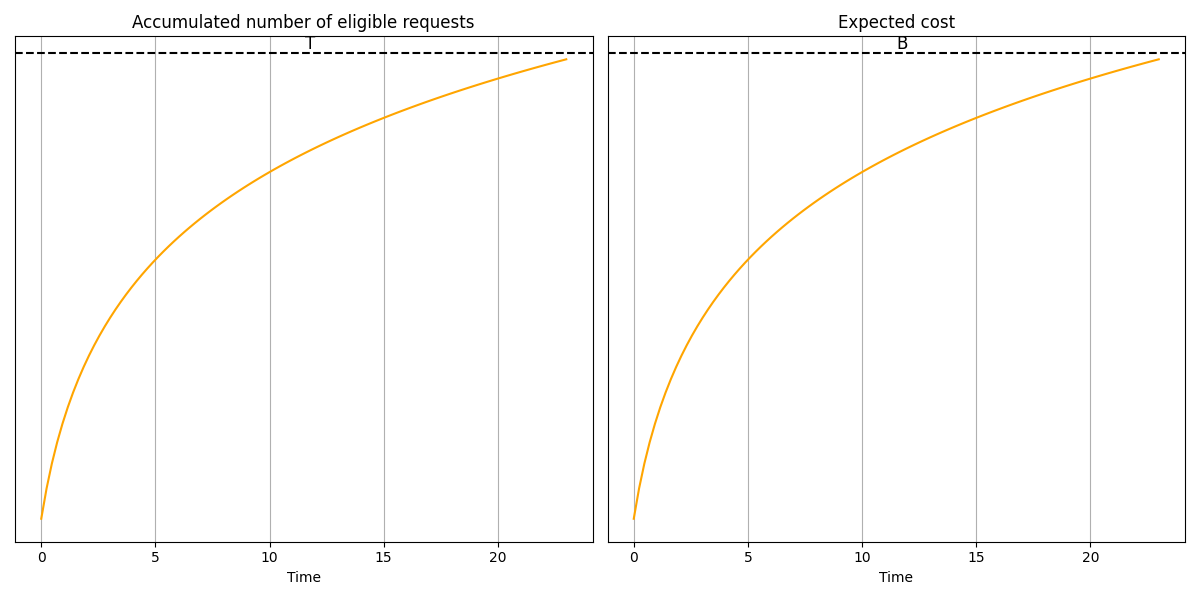
\includegraphics[width=1\textwidth]{bidding_graphs.png}
			\caption{Left: Accumulated number of eligible requests. Right:Accumulated expected cost.}
		\end{figure}
		
\end{frame}

%----------------------------------------------------------------------------------------



\begin{frame}
	\frametitle{Auto Bidding Algorithm}
	
		
		In practice, we construct an expected cost curve based on flow ratio map (e.g. 15 minute granularity):
		
		\begin{figure}[H]
			\centering
			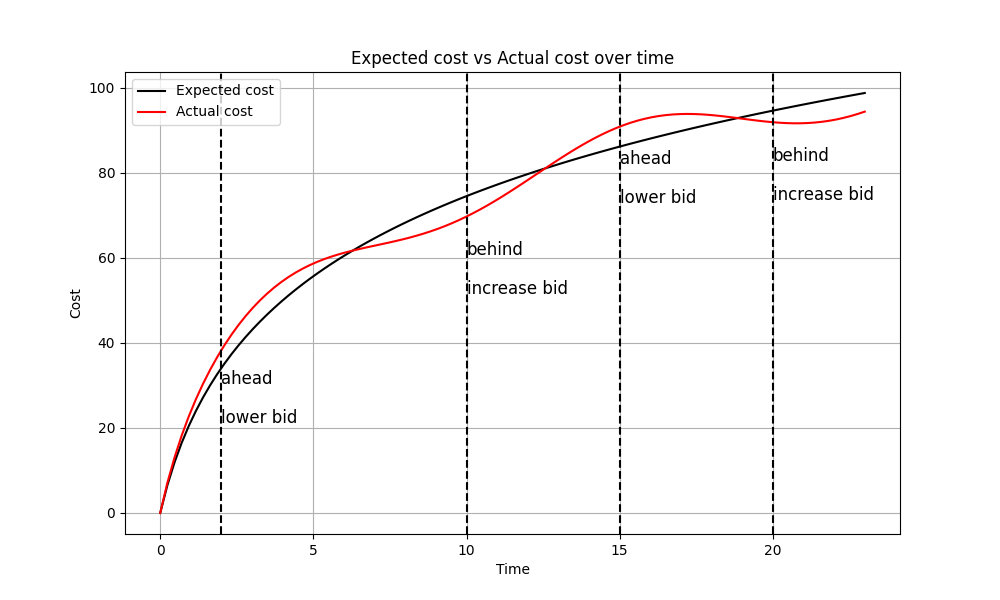
\includegraphics[width=0.8\textwidth]{flow_ratio_map.png}
			\caption{Expected cost vs Actual cost over time}
		\end{figure}
		

\end{frame}

%----------------------------------------------------------------------------------------




\begin{frame}
	\frametitle{Auto Bidding Algorithm}
	
	\begin{block}{How To Find Optimal Bid $b^*$ (cont'd)} 
	Intuitively, do pacing by comparing actual cost to expected cost:  \pause 
		\begin{itemize}
			\item Ahead schedule      $\rightarrow$ lower bid \pause
			\item Behind schedule  $\rightarrow$ increase bid \pause
			\item Ahead schedule      $\rightarrow$ lower bid \pause
			\item Behind schedule  $\rightarrow$ increase bid  \pause
		\end{itemize}
		
		By following the curve: 
		\begin{math}
			b_t \rightarrow b^*  
		\end{math}
	\end{block}
\end{frame}

%----------------------------------------------------------------------------------------
	

\begin{frame}
	\frametitle{Auto Bidding Algorithm}
	
	\begin{block}{Controller-based Algrorithm} 
		\textbf{Approach 1: PID Controller}
		\pause
		\begin{enumerate}
		\item $e(t_{k}) = C_e(t_{k}) - C_a(t_{k})$
		\\
		\pause 
		\item  $\phi(t_{k+1}) \leftarrow \lambda_P e(t_{k}) + \lambda_I \sum_{j=1}^{k} e(t_j) \Delta t_j + \lambda_D \frac{\Delta e(t_k)}{\Delta t_k}$
		\\
		\pause 
		\item 
		$b(t_{k+1}) \leftarrow b(t_k) \cdot \exp(\phi(t_{k+1}))$
	\end{enumerate}
	\end{block}
\end{frame}

%----------------------------------------------------------------------------------------



\begin{frame}
	\frametitle{Auto Bidding Algorithm}
	
	\begin{block}{Controller-based Algrorithm(cont'd)} 
	\textbf{Approach 2: MPC Controller}
	
	MPC optimizes the entire future spend, at time $t$, remaining budget $B_{t,r}$ \\  \pause  $\Rightarrow$ expected cost speed $cs_t$
	\\ \pause  
	$\Rightarrow$ expected bid price $b_t$ 

	\end{block}


	\pause

	\begin{tcolorbox}[colframe=red,colback=blue!5!white]
		\begin{center}
			\textbf{Goal:}  find $cs_t = f(b_t)$ 
		\end{center}
	\end{tcolorbox}
\end{frame}

%----------------------------------------------------------------------------------------


\begin{frame}
	\frametitle{Auto Bidding Algorithm}
	

		iMPC: fitting historical (bid, cost) pairs +  interpolation 
		
		
		\begin{figure}[H]
			\centering
			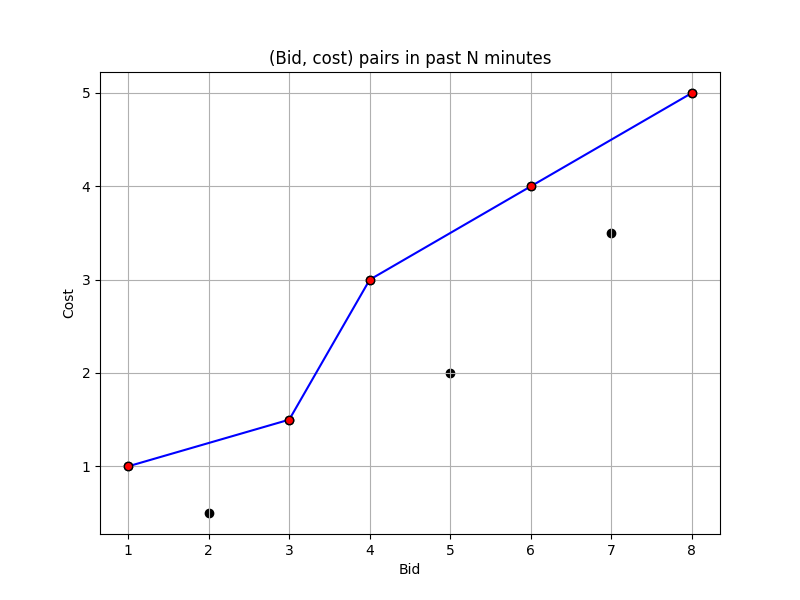
\includegraphics[width=0.6\textwidth]{bid_cost_pair.png}
			\caption{(Bid, cost) pair in past N minutes. Blue line represents the longest increasing subsequence used for interpolation.}
		\end{figure}

\end{frame}

%----------------------------------------------------------------------------------------



\begin{frame}
	\frametitle{Auto Bidding Algorithm}
	
	\begin{block}{iMPC Controller(cont'd)} 
		
			\begin{enumerate}	
			\item  At a given time, $cs_t = f(b_t)$ (non-decreasing) \pause \\
			\item  Choose longest increasing subsequence, then interpolate to get $f$ \pause \\
			\item  $b_t = f^{-1}(cs_t)$ 
			\end{enumerate}

	\end{block}

\end{frame}

%----------------------------------------------------------------------------------------



\begin{frame}
	\frametitle{Auto Bidding Algorithm}
	
	\begin{block}{MPC Controller} 
	
	Isotonic Regression based MPC
	

		
	\end{block}
	
\end{frame}

%----------------------------------------------------------------------------------------





\begin{frame}
	\frametitle{Cost Cap Algorithm}
	
	\begin{block}{Formulation(use CPC ads as example)} 
		\[
		\max_{x_t} \sum_{t=1}^{T} x_t r_t
		\]
		subject to
		\[
		\sum_{t=1}^{T} x_t c_t \leq B
		\]
		\[
		\sum_{t=1}^{T} x_t c_t \leq C \left( \sum_{t=1}^{T} x_t r_t \right)
		\]
		where $C$ is cost cap (advertiser bid)
	\end{block}
	
\end{frame}

%----------------------------------------------------------------------------------------


\begin{frame}
	\frametitle{Cost Cap Algorithm}
	
	\begin{block}{Optimal Bidding Formula} 
		Use primal-dual method, similarly we get optimal bid:
		\[
		b^* = \frac{1 + \mu^* C}{\lambda^* + \mu^*} = \frac{\lambda^*}{\lambda^* + \mu^*} \cdot \frac{1}{\lambda^*} + \frac{\mu^*}{\lambda^* + \mu^*} \cdot C
		\] \pause 
		
		\textit{Note: if $\mu^* = 0$, $b^* = \frac{1}{\lambda^*}$ which is equivalent to auto bidding} \\ 
		
		\pause
		 
		In practice, we use the "cost-min" algorithm:
		\[
		b_t = \min(\text{flow\_bid}, \text{risk\_bid})
		\]
		
		where
		\[
		\text{risk\_bid} = \frac{\text{remaining budget}}{\text{remaining event goal}}
		\]
		\text{flow\_bid} is the same as in auto-bidding.
	\end{block}
	
\end{frame}

%----------------------------------------------------------------------------------------




	

	
	
\end{document}